\documentclass[a4paper,10pt]{article} 

\usepackage[utf8]{inputenc} 
%\usepackage[T1]{fontenc}

\usepackage{textcomp}           % Extra Symbole (Grad Celsius etc.)
\usepackage{amssymb,amsmath}    % Schöne Formeln (AMS = American Mathematical Society)
\usepackage{graphicx}           % Bilder und Seitenränder
\usepackage{subcaption}			% captions for subfigures
\usepackage{booktabs}           % Schönere Tabellen
\usepackage{colortbl}           % Farbige Tabellen

%\usepackage{tcolorbox}			% schöne bunte Boxen
\usepackage{mathtools}			% \mathclap für ordentliche \underbrace-			environments
\usepackage{geometry}			% Pagelayout mit \newgeometry, \restoregeometry
\usepackage{float}
\usepackage{wrapfig}
\usepackage{enumitem}
\usepackage{float}
\usepackage{braket}
\usepackage{caption}
\input{insbox.tex}
%\usepackage{pst-optexp}
%\usepackage{auto-pst-pdf}

\graphicspath{{./img/}}


\bibliographystyle{unsrtnat}

\renewcommand{\k}{\mathbf{k}}
\begin{document}
\begin{titlepage}
 \begin{center}
	\Large{Advanced laboratory class 2}
	\end{center}
	\begin{center}
	 \LARGE{\textbf{FP2 - Amplitude and Phase modulation}}
	\end{center}
	
	\begin{center}
	
	\large Marco \textsc{Canteri} \\
	marco.canteri@student.uibk.ac.at
	\end{center}
	
	\begin{center}
	\vspace{1cm}
	Innsbruck, \today
	\vspace{2cm}
	\end{center}
	
	\begin{center}
	
\includegraphics[scale=0.4]{img/uibk} 
	\end{center}

\end{titlepage}
\begin{abstract}
In this experiment we studied three different modulation techniques: amplitude, frequency, and phase modulation. In the first part we simply generated a modulated signal with a frequency generator and analysed it with an oscilloscope. In the second part of the experiment we built an amplitude modulated signal from two different frequency generators, converted it from  electric to a light signal with an Acousto-Optical Modulator and demodulated with a photodiode before measuring it. Finally we studied the frequency response of our system.
\end{abstract}
\section{Introduction}
The experiment is divided in two parts. The aim of the first part is to study modulated signal in time and frequency domain. In order to fulfil this goal we used a very simple setup consisting of a frequency generator connected to an oscilloscope. We exploited the frequency generator features to create a modulated signal in amplitude, frequency and phase. 
For the amplitude modulated signal we measured the wave for three different AM depths and another one with a different frequency. Frequency modulation was studied for fourteen different frequency deviations, we acquired the time signal for only two frequencies, for the rest we studied only the spectrum. Finally we took one measure of a phase modulated square wave signal both in time and frequency domain.\\
For the second part we created an amplitude modulated signal from two different function generators, then we converted this electric signal into a light one using an Acousto-Optical Modulator (AOM). The light signal was later detected and demodulated with a photodiode, whose signal was analysed with an oscilloscope. We studied the frequency response of this system and we tried to determine AOM's proprieties with the phase delay.
\section{Theory}
\subsection{Amplitude modulation}
Amplitude modulation is a technique used to encode a message signal $m(t)$ into a carrier wave which is then transmitted and demodulated in order to recover the original message. Amplitude modulation, as the name suggests, consists of encoding $m(t)$ into the amplitude of a cosine wave, i.e.
\begin{equation}\label{ammodulation}x(t) = A_c (1+ m(t))\cos(2\pi f_c t),\end{equation}
In our experiment we used as message a cosine wave $m(t) = h\cos(2\pi f_m t)$, where $h$ is called modulation index. Usually $h$ is expressed as a percentage and in that case it is called AM depth.\\
The spectrum of $x(t)$ can be calculated mathematically by performing a Fourier transform on the function, but first it is better if we rewrite equation \eqref{ammodulation} with prosthaphaeresis identities
\begin{equation}x(t) = A_c \cos(2\pi f_c t) + \frac{A_ch}{2}\left[\cos(2\pi(f_c + f_m)t)+\cos(2\pi(f_c - f_m)t)\right].\end{equation}
Here the spectrum is evident, there is a peak at $f_c$ and two side peaks one on each side of $f_c$ spaced from the central peak by $f_m$, as depicted in figure \ref{amtheory}
\begin{figure}[H]
\centering
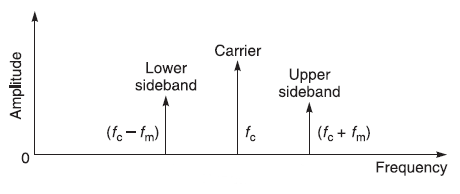
\includegraphics[width=.7\textwidth]{amtheory}
\caption{Theoretical spectrum for positive frequency}\label{amtheory}
\end{figure}
\subsection{Frequency and phase modulation}
Instead of encoding a message in the amplitude of a cosine carrier, we can encode it in the phase or in the frequency of such carrier. In the most general case $m(t)$ can be transmitted in the form
\begin{equation}x(t) = A_c \cos(2\pi f_ct + \phi(m(t))).\end{equation}
In the case of frequency modulation, we have $\phi(m(t))= a \int m(t)dt$, while for phase modulation it is simply $\phi(t) = a m(t)$. Therefore, frequency and phase modulation are strictly correlated and we can switch from one to the another taking the integral of the message. Thus, here we treat only the frequency case, but our derivations hold for phase modulation too. \\
Suppose that we want to transmit a message of the form $m(t) = A_m \cos (2\pi f_mt)$, as we do in our experiment, let us choose $a = 2\pi f_\Delta$, where $f_\Delta$ is called frequency deviation, then for the frequency modulation we have a modulated signal
\begin{equation}\label{freqmodu}x(t) = A_c \cos\left(2\pi f_ct + 2\pi f_\Delta A_m \int \cos (2\pi f_mt)\right) =  A_c \cos\left(2\pi f_ct + \frac{A_m f_\Delta }{f_m }\sin (2\pi f_mt)\right), \end{equation}
in order to simplify this equation, we define $\omega_c = 2\pi f_c,\omega_m = 2\pi f_m$ and we define the modulation index $\mu = \displaystyle\frac{A_m f_\Delta }{f_m }$. With these new definitions, we can write equation \eqref{freqmodu} as
\begin{equation}x(t) =  A_c \cos\left(\omega_ct + \mu\sin (\omega_mt)\right).\end{equation}
It is difficult to calculate the Fourier transform to obtain the spectrum, but we can rewrite our expression such that the spectrum is easier to evaluate. For this reason we can try to write $x(t)$ as a sum of cosines. First of all it is better to work with complex exponentials, so
\begin{equation}\label{complexform}x(t) = \text{Re}\left(A_c e^{i\omega_c t}e^{i\mu \sin(\omega_m t)}\right).\end{equation}
Now we notice that the second exponential has a period of $T = 2\pi/\omega_m$, therefore we can expand it as a Fourier series\footnote{If f(t) is periodic with period $T$, it holds that $f(t) = \displaystyle\sum_{n=-\infty}^{+\infty} c_n e^{i2\pi n t/T}$, where $c_n = \frac{1}{T}\displaystyle\int_{-T/2}^{T/2}f(t)e^{-i2\pi n t/T}\,dt$}:
\begin{equation}e^{i\mu \sin(\omega_m t)} = \sum_{n=-\infty}^{+\infty }c_n e^{i\omega_mn t} \qquad c_n=\frac{\omega_m}{2\pi}\int_{-\frac{\pi}{\omega_m}}^{\frac{\pi}{\omega_m}}e^{i\mu \sin(\omega_m t)}e^{-i\omega_mnt}\,dt.\end{equation}
In the integral we perform a substitution $\omega_m t = \theta \implies dt = d\theta/\omega_n$, so we obtain
\begin{equation}c_n=\frac{1}{2\pi}\int_{-\pi}^{\pi}e^{i(\mu \sin(\theta)-n\theta)}\,d\theta \equiv J_n(\mu),\end{equation}
where we recognized the integral representation of Bessel functions \cite{bessel}. Therefore we arrive at
\begin{equation}e^{i\mu \sin(\omega_m t)} = \sum_{n=-\infty}^{+\infty }J_n(\mu) e^{i\omega_mn t},\end{equation}
we can use this equation in \eqref{complexform}, which yields to
\begin{equation}x(t) =  \text{Re}\left(A_c e^{i\omega_c t}\sum_{n=-\infty}^{+\infty }J_n(\mu) e^{i\omega_mn t}\right) =\text{Re}\left(A_c\sum_{n=-\infty}^{+\infty }J_n(\mu) e^{i(\omega_c +\omega_mn )t}\right).\end{equation}
Finally we take the real part and we get
\begin{equation}\label{finalfre}x(t) = A_c \sum_{n=-\infty}^{+\infty }J_n(\mu) \cos((\omega_c +\omega_mn )t).\end{equation}
The Fourier transform is now straightforward, since it is linear. In the spectrum we will find symmetric peaks with respect to $f_c$ equally spaced by $f_m$. The heights of these peaks are proportional to Bessel functions.
\begin{figure}[H]
\centering
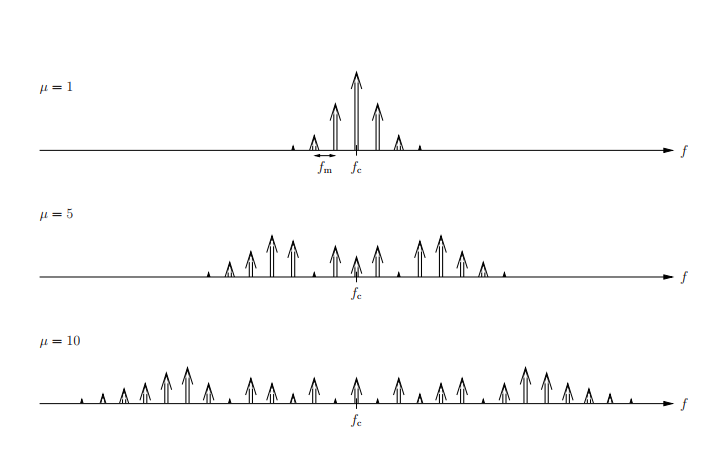
\includegraphics[width=.8\textwidth]{freqtheory}
\caption{Theoretical spectrum for positive frequency and for different value of $\mu$}
\end{figure}
\begin{figure}[H]
\centering
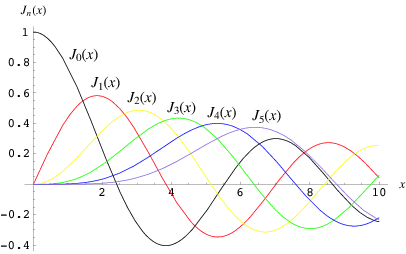
\includegraphics[width=.7\textwidth]{besseltheory}
\caption{First six Bessel functions}
\end{figure}
\subsection{Acousto-Optical Modulator}
AOM is a device that can be used to turn an electric signal into a light one. Basically it is a block of a certain material which undergoes to vibrations produced by a piezo-electric transducer. The electric signal is converted into sound waves which change the refractive index of the material such that a grating is formed. The incoming light is therefore diffracted and  changes its wavelength, intensity and phase. For our analysis it is important to focus on the phase whom the light acquire. From a bode diagram of the system it is possible to evaluate the sound speed inside the AOM from the acquired phase. Indeed the phase shift is due to the time needed from the sound wave to reach the light beam. Let us call this time $t$, and the distance that sound has to travel as $d$. Therefore, the velocity of sound is $v_s = d/t$, $d$ is a propriety of the device and can be obtained from the datasheet. $t$ can be measured from the phase shift which is in fact $\phi = 2\pi f_m t$, therefore we expect from a bode diagram a linear dependence of the phase with the frequency.
\section{Experiment setup}
For the first part of the experiment, the setup was very simple, it consisted of a function generator connected to an oscilloscope. Hence, here we will discuss only the setup for the second part. It can be found in figure \ref{setup}. The transmission part, i.e. the laser is made with an Helium-Neon laser with an output of around 1 mW at 633 nm. The laser beam is focused, with the help of two mirrors, into an AOM. We blocked the zero-th order diffracted beam, and with a lens we sent the first order in a photodiode which acts both as detector and as demodulator. The signal is created with two function generator, one used as carrier, while with the other one we generate the message to encode. These two signal were multiplied with a mixer. We measured the output of one function generator (the one we used to create the message), and the output of the photodiode with an oscilloscope.
\begin{figure}[H]
\centering
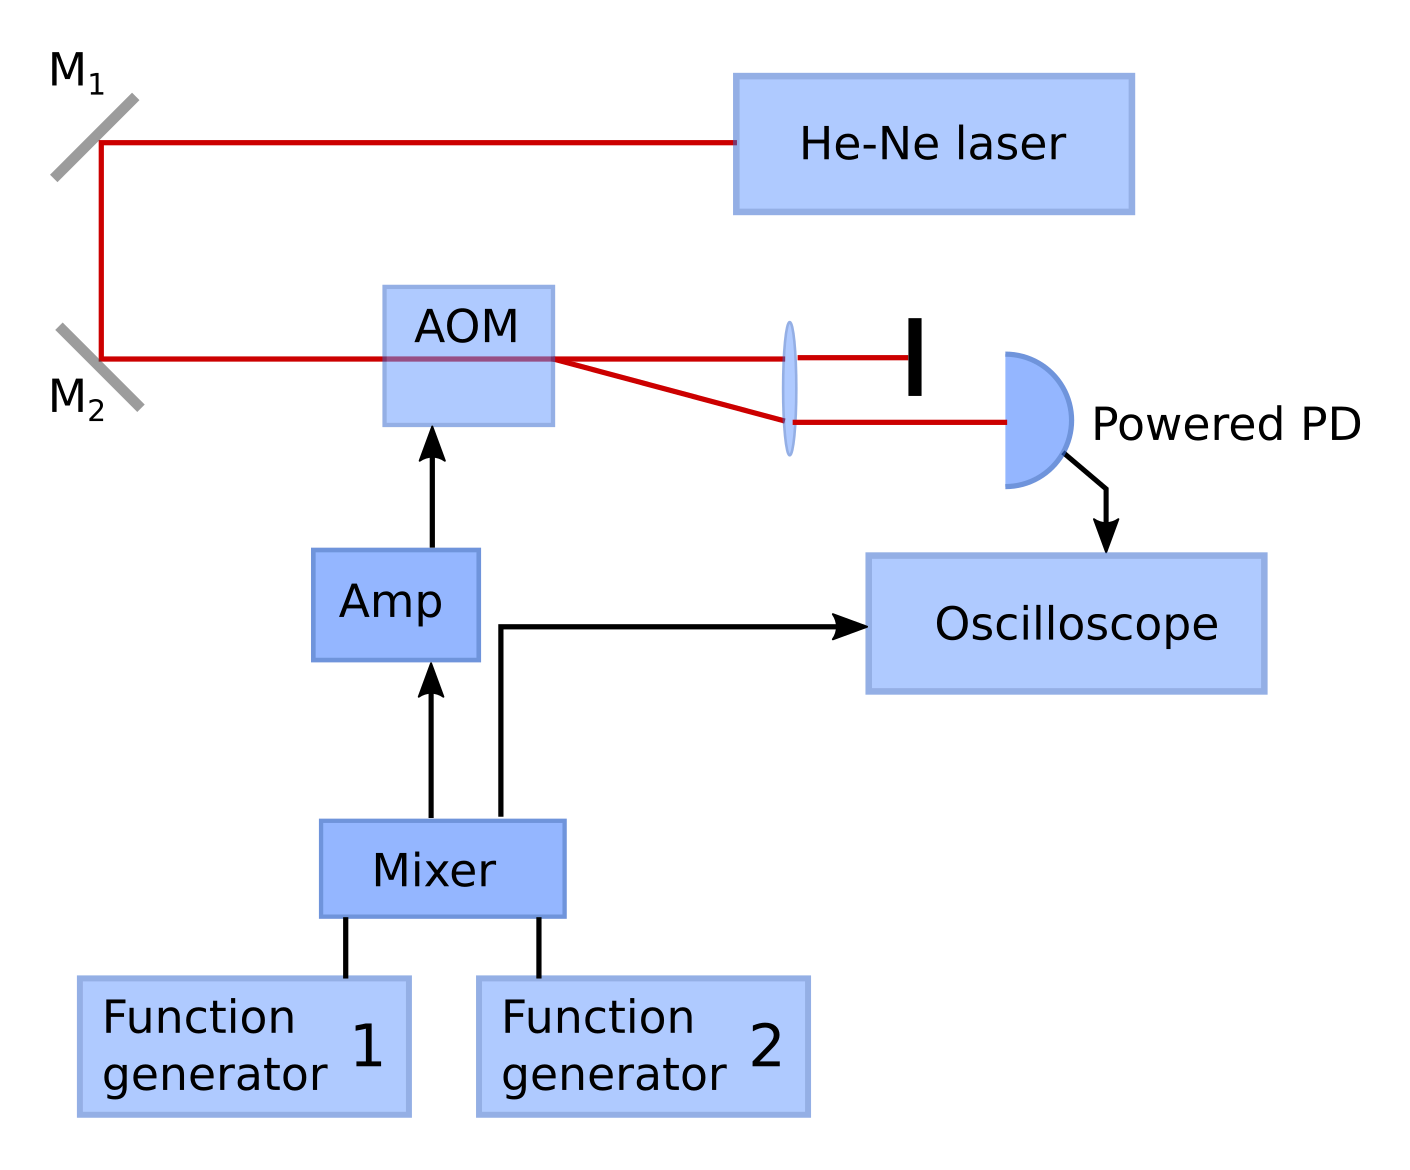
\includegraphics[width=.8\textwidth]{setup}
\caption{Setup for the second part, between the mixer and a function generator there was also a resistor used to avoid short-circuiting}\label{setup}
\end{figure}
\section{Data analysis}
\subsection{First part}
\subsubsection{Amplitude modulation}
First we studied amplitude modulation. We used as carrier a wave with amplitude $100$ mV peak-peak, and 625 kHz of frequency. We varied the frequency and the AM depth of the signal. Below  there are all four measurements in time and frequency domain. The frequency plot was obtained with the build-in Fast Fourier Transform (FFT) of the oscilloscope. In theory we should obtain infinite peaks, since they are Dirac deltas. However, in reality we obtained a broad peak, because the FFT is done with a finite number of points, and moreover we had to chose a window which cuts the signal. All this issues lead to a spectrum leakage, that is we get broader peaks. Nevertheless, we can still do some analysis, the height of the peaks depends on the FFT algorithm, but it should be at least proportional to the AM depth we chose, as can be seen from the theoretical spectrum where Dirac deltas are proportional to $h$. Furthermore, we can also check the peak frequencies.
\begin{figure}[H]
\centering
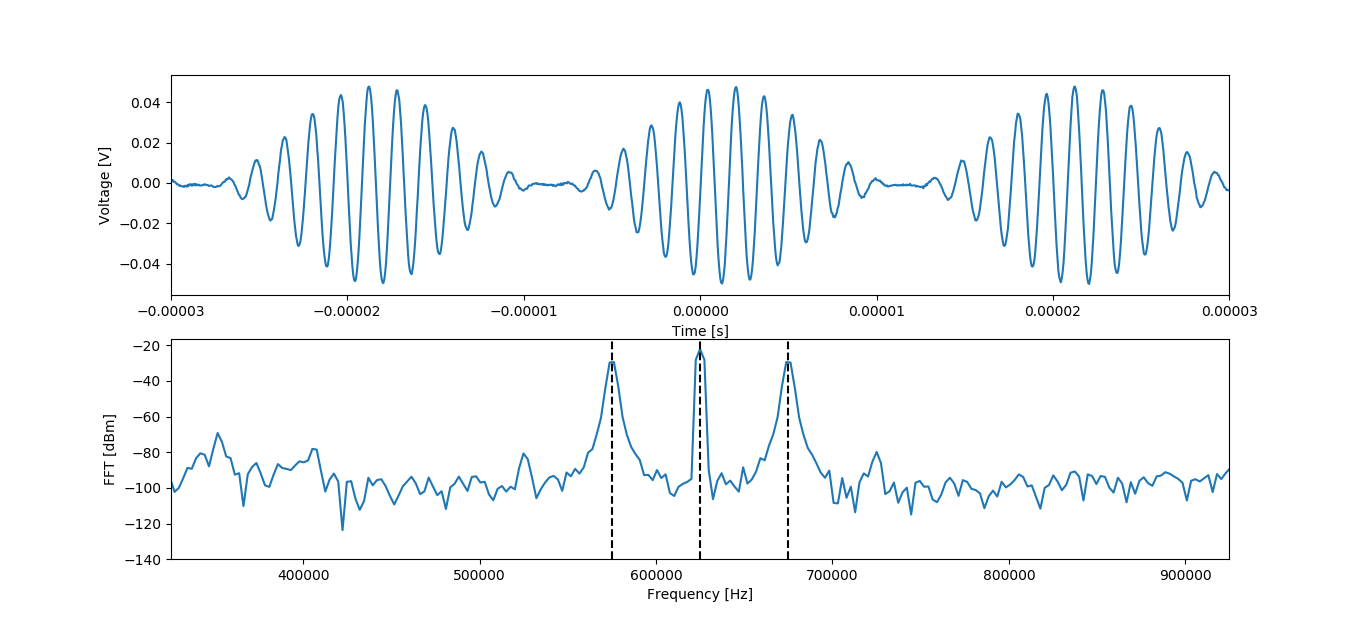
\includegraphics[width=\textwidth]{amp1}
\caption{Message frequency 50 kHz, 100\% depth. Black dashed lines plotted at 575,625,675 kHz}\label{1}
\end{figure}
\begin{figure}[H]
\centering
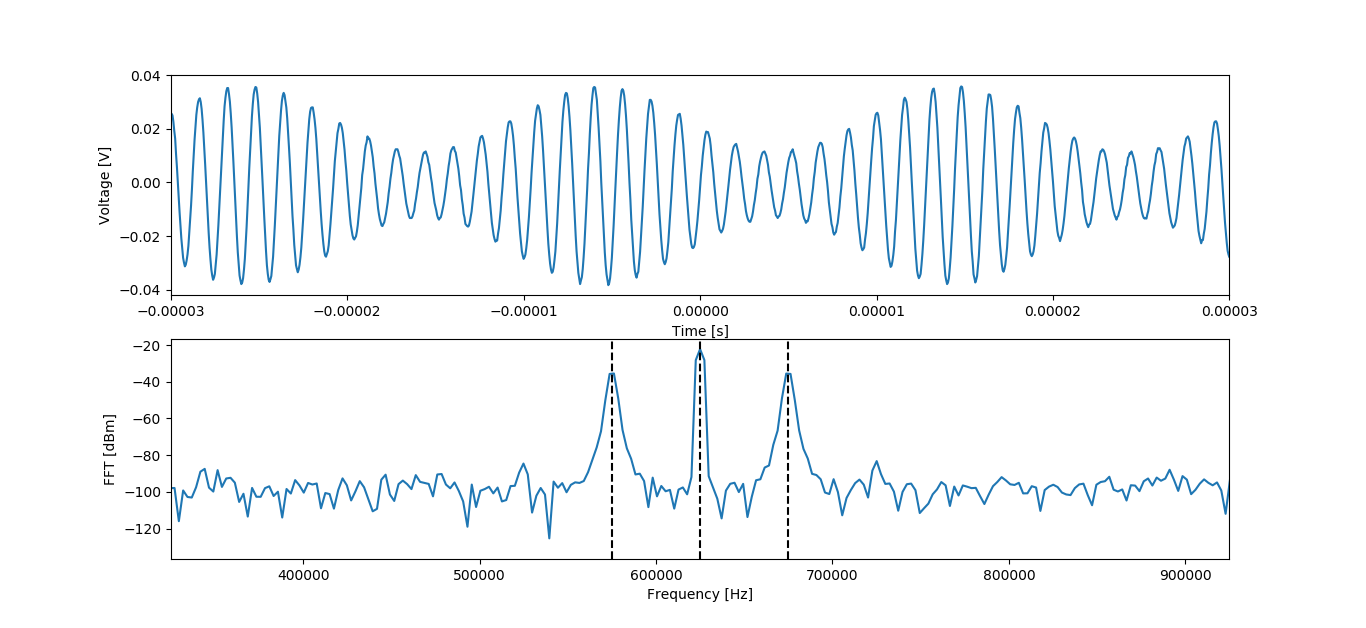
\includegraphics[width=\textwidth]{amp2}
\caption{Message frequency 50 kHz, 50\% depth. Black dashed lines plotted at 575,625,675 kHz}\label{2}
\end{figure}
\begin{figure}[H]
\centering
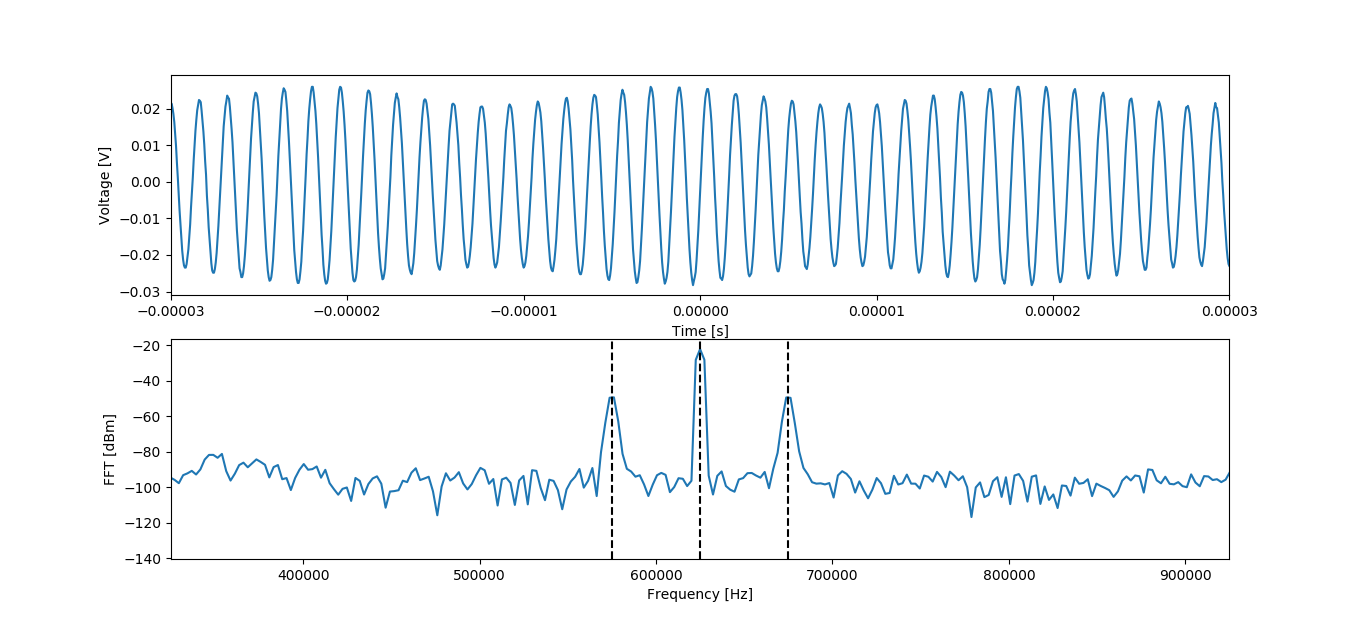
\includegraphics[width=\textwidth]{amp3}
\caption{Message frequency 50 kHz, 10\% depth. Black dashed lines plotted at 575,625,675 kHz}\label{3}
\end{figure}
\begin{figure}[H]
\centering
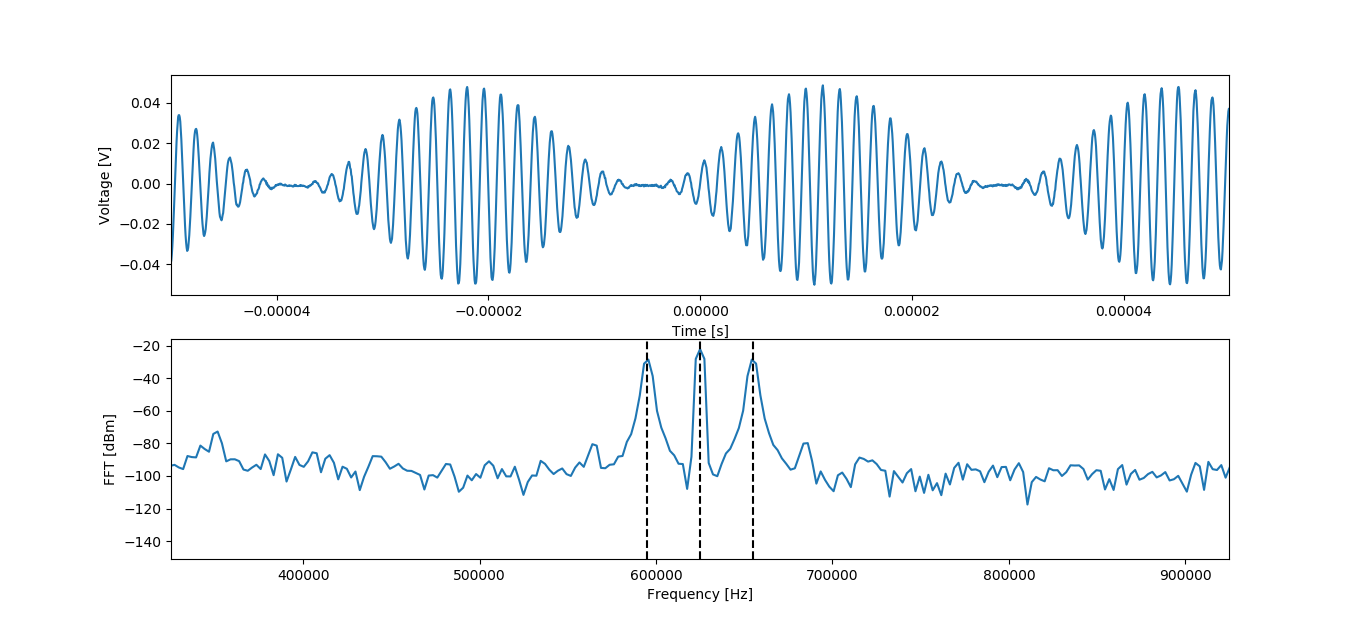
\includegraphics[width=\textwidth]{amp4}
\caption{Message frequency 30 kHz, 100\% depth. Black dashed lines plotted at 595,625,655 kHz}\label{4}
\end{figure}
From the figures it is clear that the peaks are centred at the expected frequencies. We extracted the peak heights from the data and summarized them in the following table
\begin{table}[H]
\centering
\begin{tabular}{c|c|c|c|c}
 Figure \# & left peak [dBm] & central peak [dBm]& right peak [dBm]& AM depth\\
  \hline
  \ref{1} & -29.4654 & -22.2054 & -29.4854 & 100\%\\
  \hline
  \ref{2} & -35.4854 & -22.2054 & -35.5254 & 50\%\\
  \hline
  \ref{3} & -49.3654 & -22.2054 & -49.4254 & 10\%\\
  \hline
  \ref{4} & -28.6454 & -22.2054 & -28.6454 & 100\%\\
  \hline
\end{tabular}
\caption{Height of the three peaks showed in figures \ref{1}-\ref{4}, first column is a reference to the figure}
\end{table}
From this table we can notice two interesting behaviours. First of all the height of the central peak never change, this is expected. In fact the central peak is at the carrier frequency and therefore it represent the carrier wave, we never changed it, so this peak has not changed accordingly. Furthermore, we notice that the heights of the side peaks behave as predicted, they are proportional to the depth, if the AM depth decreases, the height decreases as well. The height of the right peak is slightly greater than the left one, this is weird since they should have the same height. This behaviour can be probably explained as a systematic error introduced in the FFT algorithm or it could be due to the quantization of the frequency and therefore the algorithm to find the maximum fails. As further investigation it is possible to test different algorithms. Lastly, we see that the heights of the peaks associated with 100\% AM depth are slightly different, those measurements are made on signal of different frequency, respectively 50 and 30 kHz, therefore this difference could be explained as a different number of points involved in the FFT algorithm, since we did not change the time window used to perform the FFT.
\subsubsection{Frequency modulation}
The same analysis of the amplitude modulation, which we have just explained, was used in the analysis of the frequency and phase modulated signal. The carrier wave was the same as for the amplitude modulation. The message had a frequency of 50 kHz, and we changed the frequency deviation from 5 kHz to 200 kHz, with different steps. We report here only the two measurements for the frequency modulation where we acquired both the time and frequency domain. We will show later some of the remaining spectra which have the most interesting features.
\begin{figure}[H]
\centering
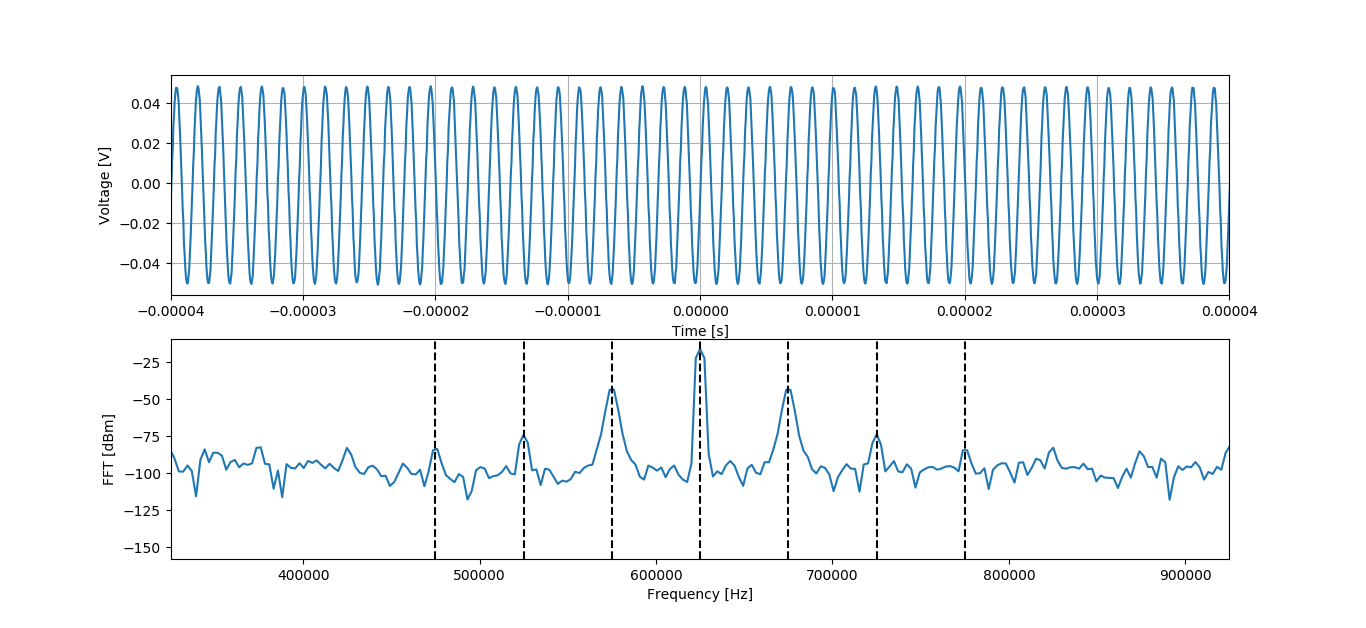
\includegraphics[width=\textwidth]{freq1}
\caption{Frequency deviation 5 kHz. Black dashed lines are plotted at $625\pm n50$ kHz for $n\in\{-3,-2,-1,0,1,2,3\}$}\label{freq1}
\end{figure}
\begin{figure}[H]
\centering
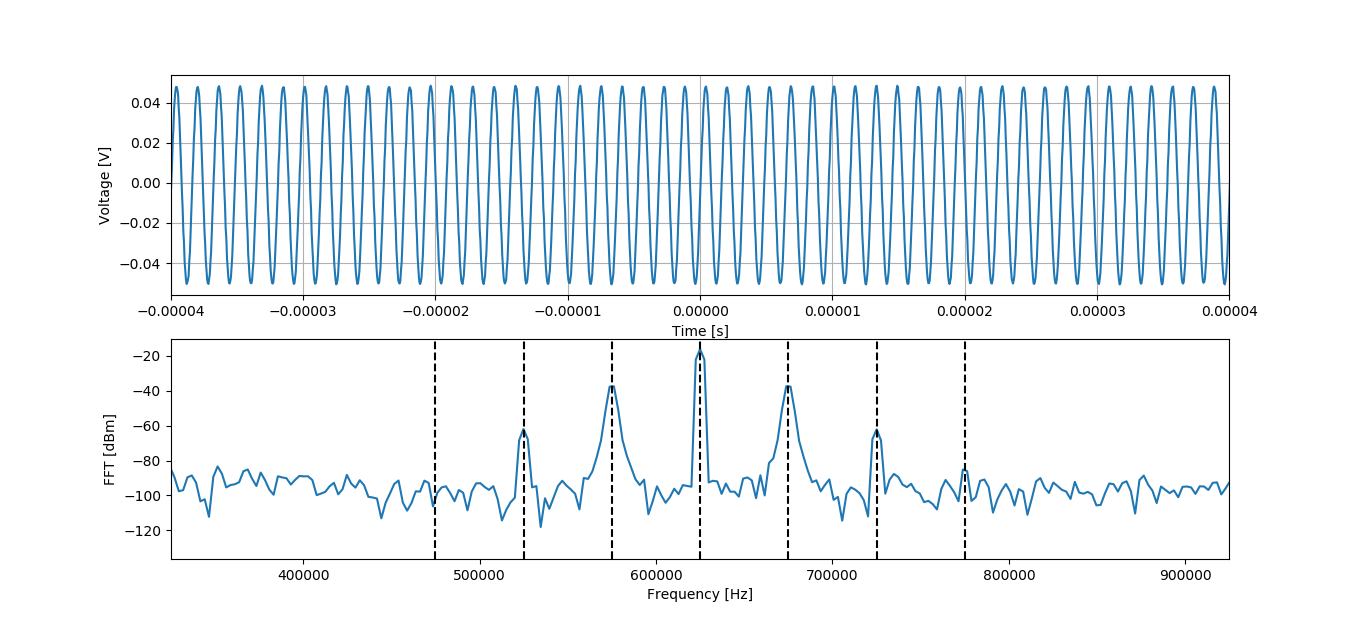
\includegraphics[width=\textwidth]{freq2}
\caption{Frequency deviation 10 kHz. Black dashed lines are plotted at $625\pm n50$ kHz for $n\in\{-3,-2,-1,0,1,2,3\}$}\label{freq2}
\end{figure}
We can see from figure \ref{freq1} and \ref{freq2} that the peaks related to the first three terms of equation \eqref{finalfre} are clearly visible, the forth peak starts to become very low and difficult to distinguish from noise. The peaks are centred at the expected frequency.
\begin{figure}[H]
%\centering
\hspace{-4.5em}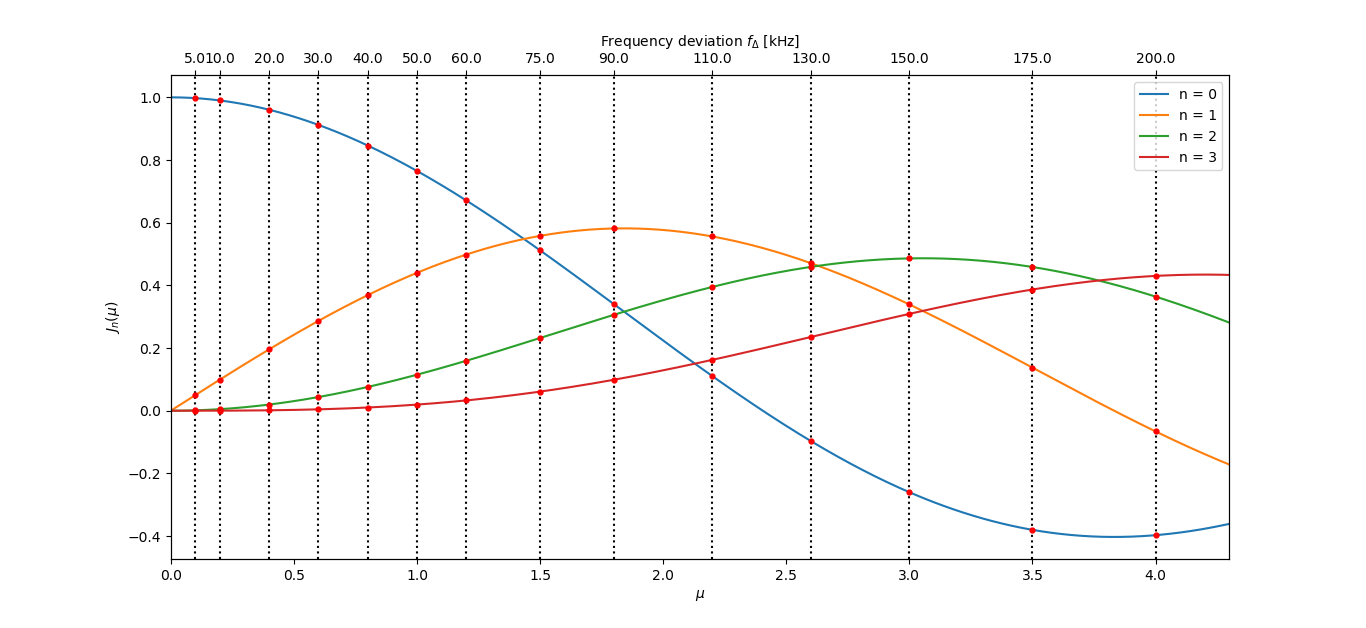
\includegraphics[width=1.2\textwidth]{bessel}
\caption{First four Bessel functions plotted as a function on $\mu$, the upper scale is $\mu$ scaled with respect to the frequency deviation $f_\Delta$. The black dashed lines are the fourteen measurements we took}\label{bessel}
\end{figure}
For analysing the peak height, which is related to Bessel functions, we plot in figure \ref{bessel} the first four Bessel functions with the modulation index  $\mu$. From this figure we can draw interesting conclusions, for instance, the central peak, i.e. the peak corresponding to $n=0$ is higher then the other for frequency deviations up to $\simeq 70$ kHz, for our measurement at 75 kHz, the central peak starts to become smaller than the second peak $n=1$ as can be barely seen in figure \ref{freqdev75}. The height difference is more pronounced at $f_\Delta = 90$ kHz, where the peak relative to $n=1$ is higher then the central peak. At $f_\Delta = 150$ kHz, we have another behaviour, the peak corresponding to $n=2$ is higher then the peak for $n=1$ and even higher then the central peak which is now the lowest one. This can be seen in figure  \ref{freqdev150}. And finally for $f_\Delta = 200$ kHz, the peak for $n=3$ is now higher then the peaks for $n=1$ and $n=2$, the central peak is now similar to $n=3$, because, although the Bessel function is negative, what it is important for the FFT is the square of the absolute value. Below there are the plots of the acquired spectra that we have just discussed.
\begin{figure}[H]
\centering
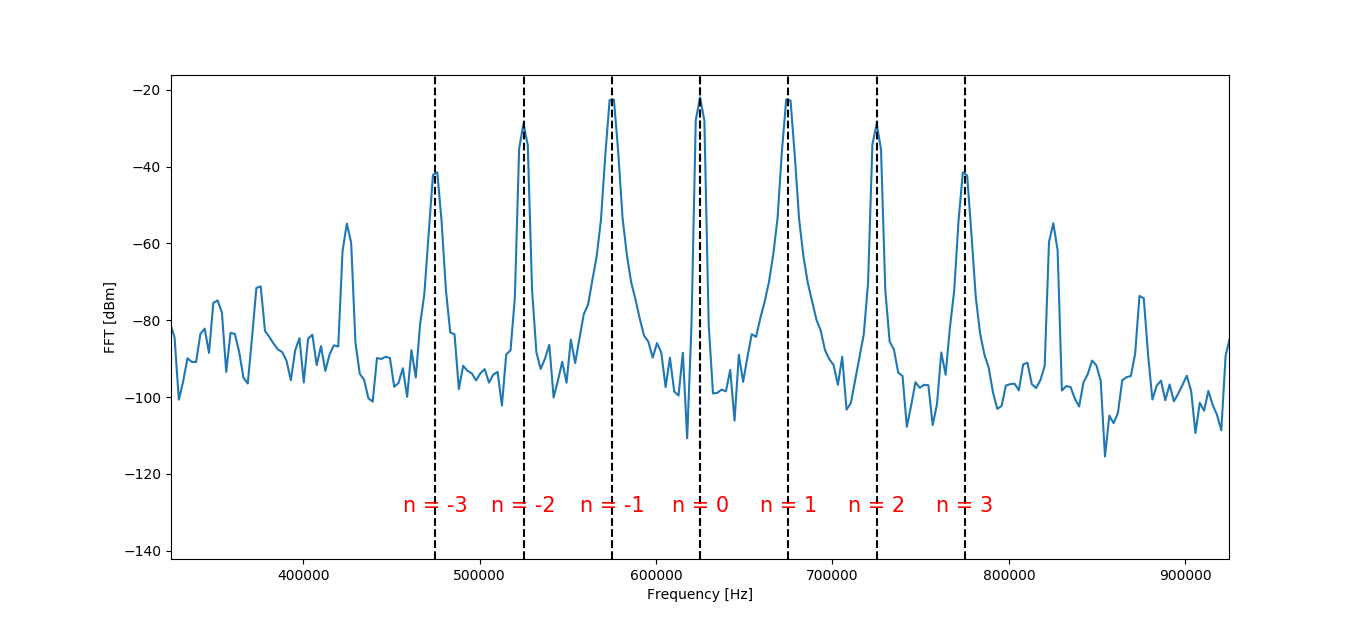
\includegraphics[width=\textwidth]{freqdev75}
\caption{Frequency deviation 70 kHz. Black dashed lines are plotted at $625\pm n50$ kHz for $n\in\{-3,-2,-1,0,1,2,3\}$}\label{freqdev75}
\end{figure}
\begin{figure}[H]
\centering
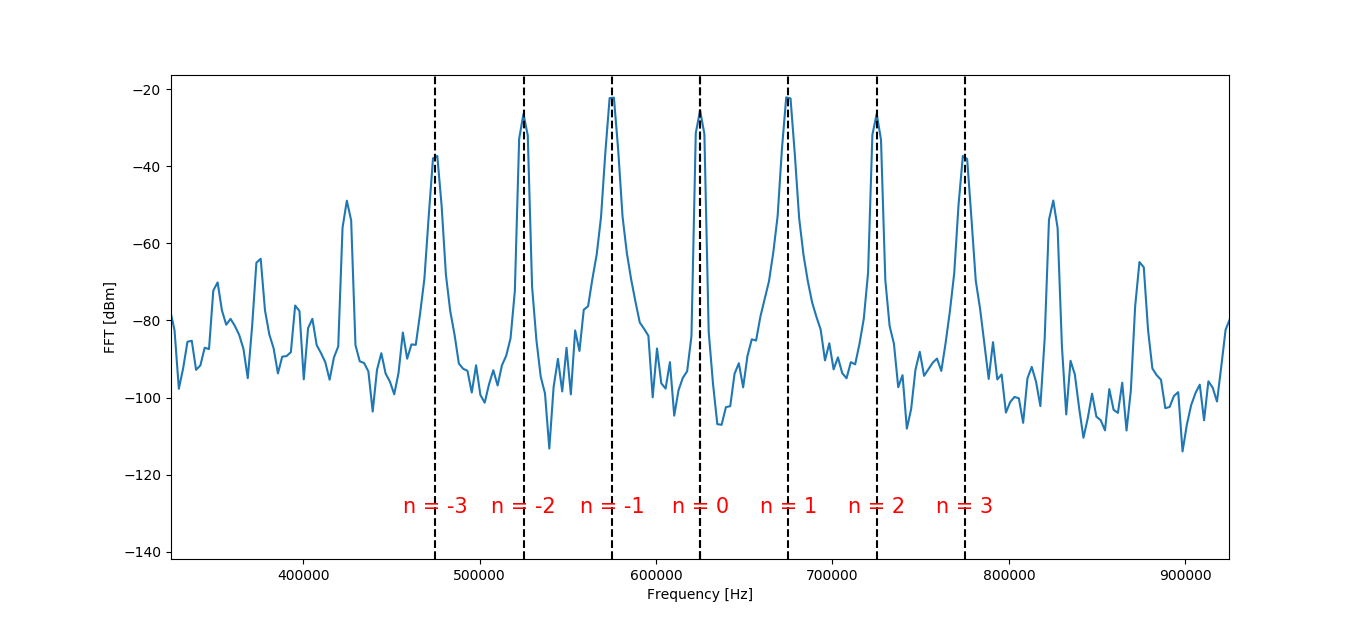
\includegraphics[width=\textwidth]{freqdev90}
\caption{Frequency deviation 90 kHz. Black dashed lines are plotted at $625\pm n50$ kHz for $n\in\{-3,-2,-1,0,1,2,3\}$}\label{freqdev90}
\end{figure}
\begin{figure}[H]
\centering
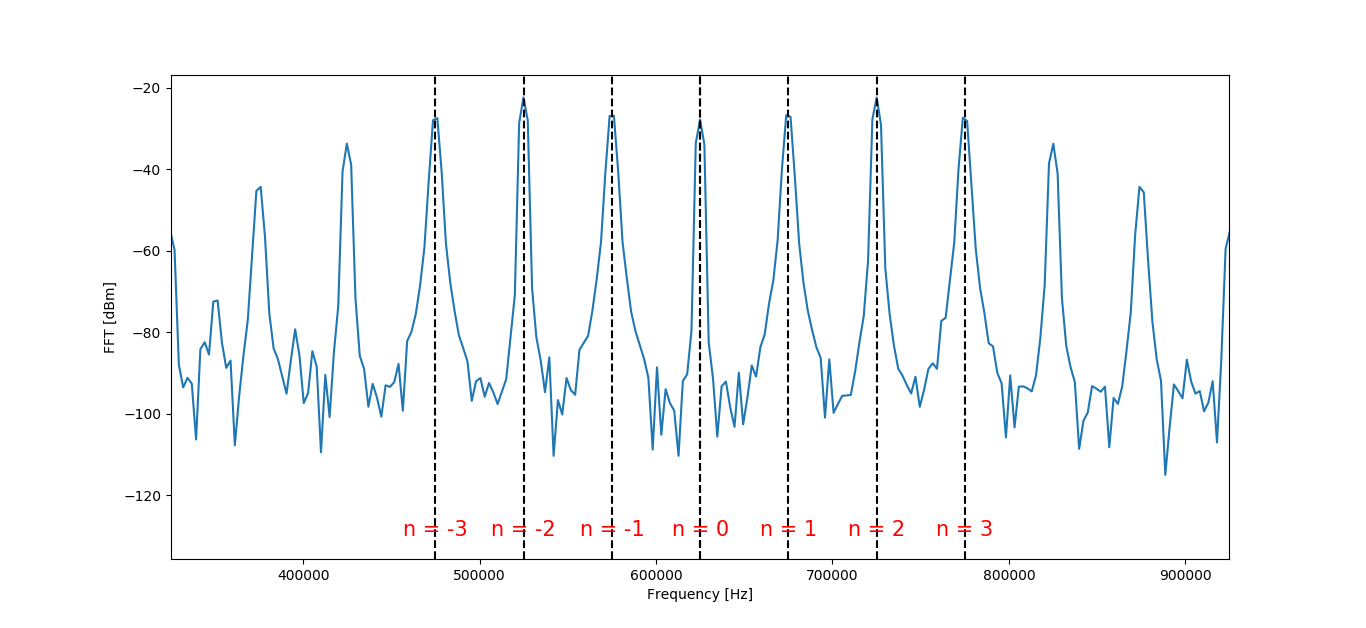
\includegraphics[width=\textwidth]{freqdev150}
\caption{Frequency deviation 150 kHz. Black dashed lines are plotted at $625\pm n50$ kHz for $n\in\{-3,-2,-1,0,1,2,3\}$}\label{freqdev150}
\end{figure}
\begin{figure}[H]
\centering
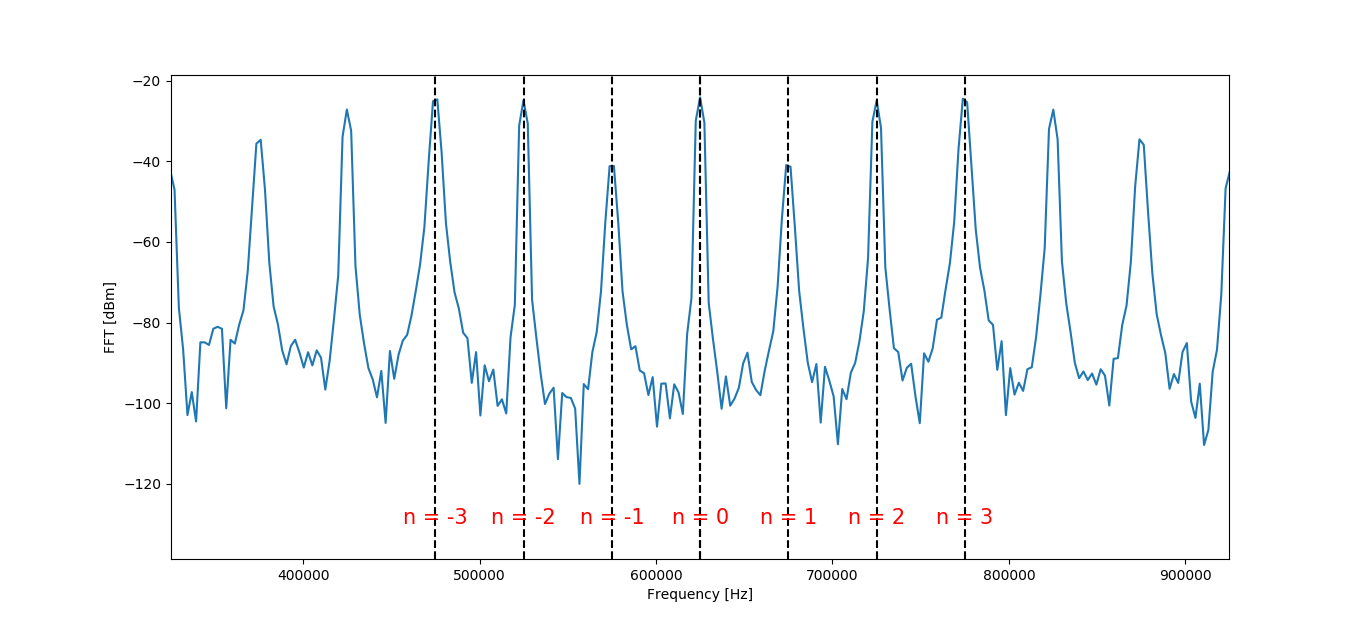
\includegraphics[width=\textwidth]{freqdev200}
\caption{Frequency deviation 200 kHz. Black dashed lines are plotted at $625\pm n50$ kHz for $n\in\{-3,-2,-1,0,1,2,3\}$}\label{freqdev200}
\end{figure}
\subsubsection{Phase modulation}
Phase modulation is very similar to frequency modulation as already said, therefore we acquired only one measurement for a phase modulated signal. We used the same carrier as for amplitude and frequency modulation, for message we used a square wave of frequency 50 kHz. The plot is in figure \ref{phase}. We can notice the sudden change in the phase of the wave, which corresponds to the square wave switching from low to high. The spectrum is very populated due to the square wave which has a lot of frequencies when written in Fourier series. The peaks are as expected spaced by 50 kHz.
\begin{figure}[H]
\centering
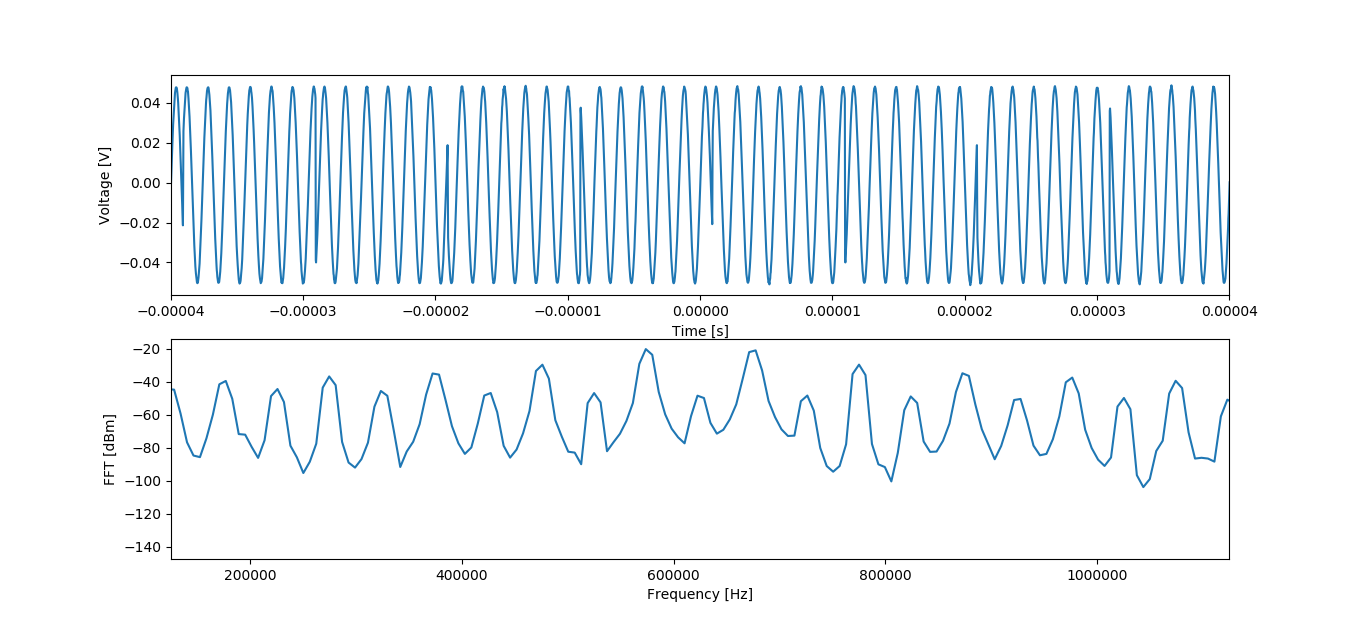
\includegraphics[width=\textwidth]{phase1}
\caption{Phase modulated signal}\label{phase}
\end{figure}
\subsection{Second part}
For the second part of the experiment we analysed the frequency response of the system in figure \ref{setup}. Therefore, we measured the bode diagram of the system, i.e. the complex quantity $H = V_{out}/V_{in}$, where both $V_{out}$ and $V_{in}$ were measured with the same oscilloscope. $V_{out}$ is the electric signal of the photodiode, while $V_{in}$ is the output of one function generator (the function generator that was the message). The complex numbers $H$ were measured by taking the amplitude of the signals and their phase difference calculated with the oscilloscope. The error is calculated as the difference between the maximum and minimum value divided by two.
\begin{figure}[H]
\centering
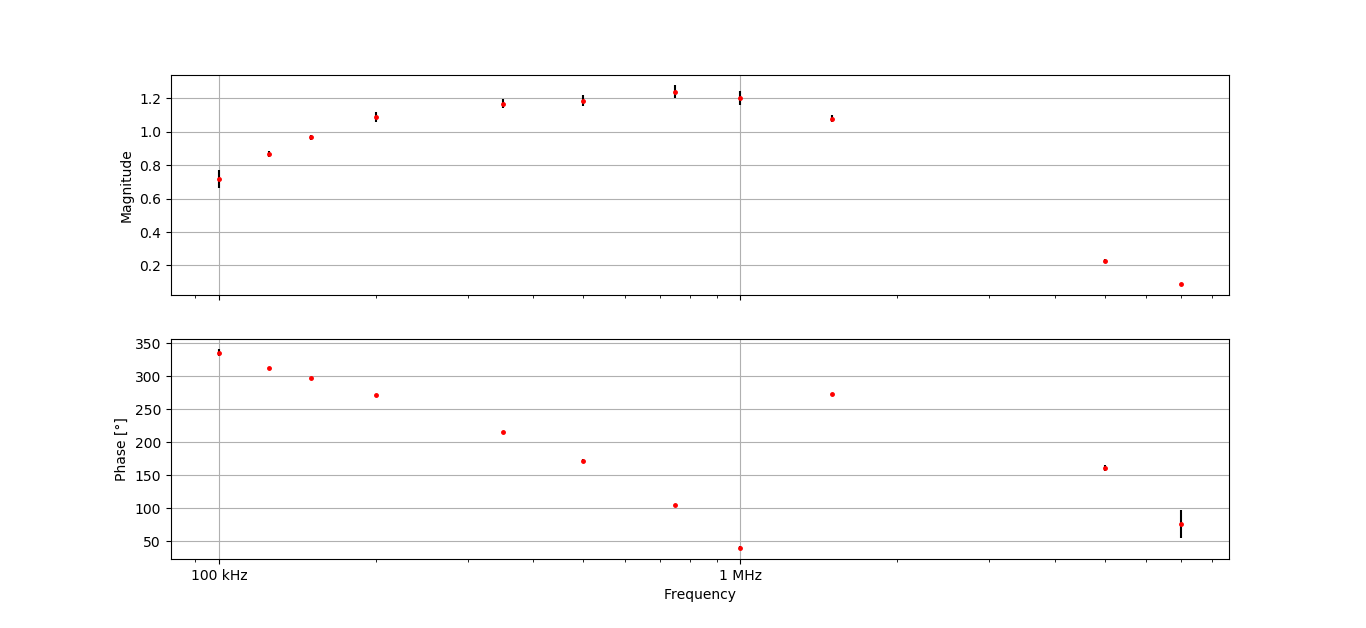
\includegraphics[width=\textwidth]{bode}
\caption{Bode diagram, the upper plot shows $|H|$, while the lower one is the phase of $H$. Red points are experimental data, the error is displayed with a black line which is not always visible}\label{bode}
\end{figure}
At low frequency we have a limitation of the mixer, which has losses for frequency under $100$ kHz. Then the system works well until some MHz, where the signal is cut again. At higher frequencies there is a low pass filter behaviour, this is due to the demodulation of the signal where a low pass filter is needed.
The phase difference is due to the brief time that the sound wave takes to reach the laser beam inside the AOM. Indeed, the sound speed inside the AOM is finite and it takes a while for the sound to go from one side to the center of the device, where it encounters the laser beam. Indeed, we can estimate the sound speed $v_s$, the phase accumulated is $\phi = 2\pi f_m t$. Therefore, since $t = d/v_s$, where d is the distance, we obtain $\phi = 2\pi f_m d/v_s$, but since the phase difference is measured only in multiple of $2\pi$, we actually have
 \begin{equation}\phi = 2\pi f_m d/v_s \mod 2\pi.\end{equation}
In figure \ref{bode}, a jump can be observed indeed. However it is not clear the linear dependence of the phase, since the plot is in logarithmic scale. We can plot $t$ as a function of the frequency $t = \phi/2\pi f_m$ and we should find an horizontal line, since the time should be always equal. 
\begin{figure}[H]
\centering
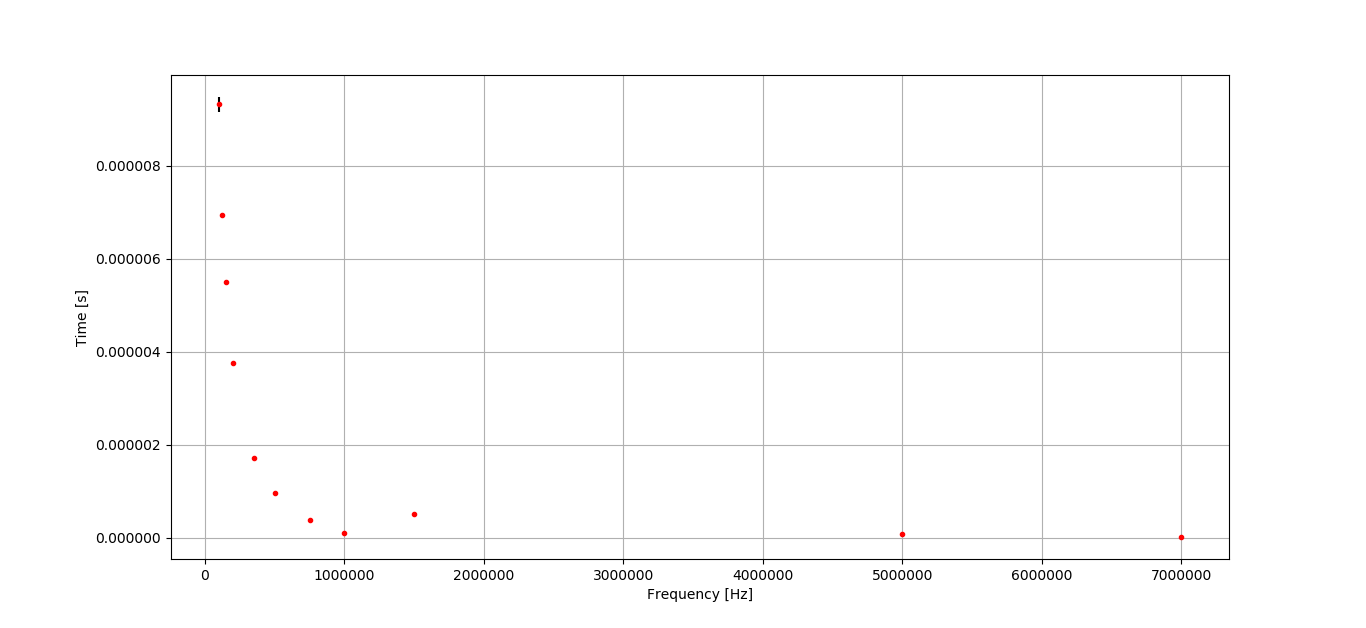
\includegraphics[width=\textwidth]{time}
\caption{Time delay which cause our phase $\phi$ as a function of the frequency}\label{cazzo}
\end{figure}
This is not our case unfortunately as can be seen in figure \ref{cazzo}. Below 1 MHz, the time changes significantly, which is not what we expect. It is possible that in that particular region of frequencies, another phase is introduced, maybe from the mixer, which does not work as it should be at low frequency.  Therefore it is not possible with our data to estimate the sound speed inside the AOM.

\section{Summary and conclusion}
In this experiment we studied three different kind of modulation: amplitude, frequency, and phase. First we focused our attention to the spectrum and we analysed the peaks. We did a qualitative analysis on such peaks, we could improve it by developing a more complete mathematical theory of spectral leakage. Just to give some insights, what we are doing during an FFT is basically multiplying the signal $x(t)$ by a window function $w(t)$, hence, instead of $x(t)$ we have the spectrum of $w(t)x(t)$. The Fourier transform of a multiplication in time can be written as a convolution in frequency, so we have $\mathcal{F}(w(t)x(t)) = \mathcal{F}(w(t))*\mathcal{F}(x(t))$, depending on the form of $w(t)$, this could be easy or not to work out analytically. When the theoretical spectrum is obtained, a fit could be done and it would be possible to compare the parameters of the fit with the values set on the function generator.\\
In the last part of the experiment we build a setup which allowed us to transmit an amplitude modulated signal we studied the frequency response and we tried to explain the limitation of our setup. Lastly we have also tried to estimated the sound speed inside the AOM, but without success. The analysis done shows that at certain frequency, the phase introduced by our system is not what we would expect from the delay to the finite sound speed. Hence, it is possible that there are other phase in our system which we did not consider in our analysis. For instance a phase could be introduced by the mixer.

\begin{thebibliography}{99}
\bibitem{bessel}
\textsc{Temme, Nico M.}, \textit{Special functions: an introduction to the classical functions of mathematical physics}, (2. print. ed.). New York 1996, Wiley. pp. 228–231. 
 \bibitem{signaltheory}
 http://www.commsys.isy.liu.se/TSDT03/material/ch5-2007.pdf
\bibitem{skriptum}
Fortgeschrittenenpraktikum 2, \textit{Excercise FP2-08: Amplitude and phase modulation}.
\end{thebibliography}
\end{document}
